

\chapter{Installation and Commissioning}
\label{ch:install}

%%%%%%%%%%%%%%%%%%%%%%%%%%%%%%%%%%%%%%%%%%%%%%
\section{Introduction}

%\fixme{I did not replace this section; Joe's new one looked identical to the orig modulo the fixmes, which I added in. AH}

This chapter discusses the LAr-FD Installation and Commissioning system's activities and responsibilities.  
LAr-FD construction and installation will occur in a series of distinct phases:

\begin{itemize}
\item installation planning and prototyping
\item surface storage identification and operation
\item excavation and outfitting of the cavern; this activity is the responsibility of the Conventional Facilities subproject (CF), 
\item construction and installation of the cryogenics system and cryostats by a construction management firm; this activity is the responsibility of the cryogenics system 
\item construction of LAr-FD components at collaborating institutions and shipment to the Far Site
\item installation of detector components and installation management
\item commissioning activities leading to CD-4
\end{itemize}

The Installation and Commissioning system will accept responsibility for the LAr-FD cavern, associated tunnels, infrastructure and above-ground facilities from Conventional Facilities upon completion of the Conventional Facilities contract. The cavern will be outfitted with the following utilities upon receipt of beneficial occupancy:

\begin{itemize}
\item ventilation in accordance with OSHA standards
\item electrical power sufficient for the HVAC, cryogenics plant cooling and general 110-V service
\item quiet power for the electonics with a double Faraday-shielded transformer located some distance from the cavern to take advantage of the inductance of the power lines. The primary shield will be connected to the main substation via a grounded feed wire and the secondary shield will be connected to the Ufer ground.
\item communications consisting of telephone lines and computer network
\item cavern lighting in accordance with OSHA regulations for industrial use
\item tunnel lighting with battery-powered backup or emergency circuit backup
\item environmental monitoring of oxygen, carbon monoxide, smoke and temperature
\item dual isolation bulkheads separating the cavern from the existing Far-Site facility
\item sump pumps for groundwater removal
\item over head conveyances
\end{itemize}

After beneficial occupancy of the completed cavern from the 
CF subproject, the cavern ventilation system will be tested to assure adequate performance with regard to ODH requirements. The system will be tested with oxygen monitors distributed around the cavern and a controlled argon spill. Remedial action will be taken if required during cryostat and cryogenics construction.

The cryostat and cryogenics contractor will retain responsibility for the site during construction of the cryostat and cryogenics system. The Cryostat and Cryogenics System group will provide oversight during this phase. Upon completion of this contract, the facility will be in the following state:

\begin{itemize}
\item the LN2 refrigeration system will be constructed and commissioned with liquid nitrogen
\item the LAr systems and cryostats will be constructed and tested without the introduction of cryogens \item the access hatches on the cryostat and the cryostat feedthroughs will be temporarily sealed
\item the APA- and CPA-installation support beams will be in place
\item the cryostat will be connected to the steel roof structure thus connecting the detector ground to the Ufer ground
\end{itemize}

The detector will utilize the cryostat pit rock bolts as part of the grounding scheme. The rock bolts in the pit will extend through the shotcrete that lines the cavern and be attached to the reinforcing steel network within the cryostat concrete liner, forming an Ufer ground. The reinforcing steel will be connected to the steel truss cover. The Ufer ground will be connected to the detector ground (the cryostat SS liner) through a low-impedance connection.

The Installation and Commissioning group will be responsible for all LAr-FD-related activities at the Far Site from this point in time until the end of the LAr-FD project. Close coordination is clearly required between this group, system groups that provide components and other Far Site construction activities. 

On-project commissioning activities include the coordination of system-checkout activities, culminating in the approval to introduce LAr into the detector modules, and managing the steps required to meet the CD-4 goals. 

\fixme{Where is reference in text to this figure?}
\fixme{Note to author who puts in new figures: Please use the new `cdrfigure' environment. I've inserted a model just below each existing `figure' env.  Notice the label within the cdrfigure environment is ``tpc-in-two-cryostats'' but the reference needs to point to ``fig:tpc-in-two-cryostats'' (with the fig: in it) }


%%%%%%%%%%%%%%%%%%%%%%%%%%%%%%%%%%%%%%%%%%%%%%
\section{Integration - Permanent Equipment}
\label{fd:install:integ}

The Installation and Commissioning system will provide some permanently installed equipment that is 
used by multiple Detector systems or is integral to the installation process.  This equipment includes the 
relay racks, cable management, support rails for the TPC and the remaining outfitting of the detector 
cavern that was too detector-specific to be included with the conventional facilities work.

%%%%%%%%%%%%%%%%%%%%%%%%
\subsection{Relay Racks and cable management}
% (Howell)
\label{fd:install:integ:racks}

A port is located above every other APA junction and each port will serve the two upper APAs located directly underneath it. Cables for the lower two APAs will be routed from ports adjacent to the outer edge 
of the cryostat.  The cables will travel down enclosed cable trays on the two side walls of the cryostat to the floor and over to the closest rows of APAs.  Cables for the other row of APAs will be routed similarly 
down the opposite side wall.  The horizontal portion of the cable run will be outside of the wire planes, so the use of double shielded cable such as Amphenol skew clear may be adequate. If not, then custom metal shields will be mounted on the front-end circuit boards. 

The racks will be mounted either directly over the ports or adjacent to them with an extension to the rack that covers the port. All cables can be brought out of the cryostat into a grounded and shielded 
enclosure.. The plan is to use 36-in-deep racks and construct a shielded area on the back side of the rack to hold and shield the excess cable. 28 racks will be required for each cryostat, and rack space will be shared between the TPC and photon-detection system readout and power supplies. 

A modest number of racks will be required for the DAQ. Two options are under consideration for the location main DAQ racks. One option would transport data on fibers to the surface as quickly as possible 
with the main DAQ racks may be located on the surface near a control room. The second option locate all DAQ racks underground with an environmental enclosure for the rack. For the second option a small adjoining control room would also be located underground.

All relay racks will be equipped with rack protection and monitoring. The racks will be supplied by the 
detector installation effort along with the labor to develop the rack plan.

%%%%%%%%%%%%%%%%%%%%%%%%%
\subsection{Detector Electrical Ground} 
\label{fd:install:integ:elecgnd}
%\fixme{material from Marvin , docdb 7310}

The LAr-FD will have approximately 200,000 channels of electronics with an intrinsic noise level of less than 1,000 electrons. These channels will be connected to wires that are seven meters long. Thus, 
grounding, shielding and power distribution are critical to the success of the experiment. In the reference design the entire detector pit will be treated as the detector ground for the following reasons: 
For the purpose of maintaining a low-noise performance within each of the proposed cryostat detectors, the construction of the LBNE far detectors' grounding system requires that there be separate grounding 
structures for the cryostat tank walls and for the cavern and its utilities. Both the cryostat detectors and the cavern structures will employ an Ufer ground, or concrete encased grounding electrodes, within the concrete construction. The guiding principle for the LBNE far detector's grounding system is to minimize, 
as much as possible, any ground currents from flowing between the AC power distribution system and the detector cryostats. Also, any flow of ground currents, both conducted and coupled, need to be 
minimized between the individual detector cryostats. Therefore, there are specific requirements for the connection and spacing of the reinforcing metal bars (rebar) set in the concrete for the cryostats' 
construction and for the specific and controlled interconnections between these separate grounding structures.

There shall be electrical separation between the cavern's rebar/concrete/shot-crete construction and the cryostats' rebar/concrete construction. The rebar of one structure and the rebar of the other structure 
shall not come in direct contact with each other. The rebar for all four vertical walls and the cryostat floor concrete shall be integrated together in order to form a uniform grounding structure between all five 
concrete cryostat surfaces. The top plate of each cryostat detector shall serve as the detector's grounding point and be connected uniformly to the detector's Ufer ground structure.

Since the cavern will be cored out of solid rock, there will be no integrated metal "building" support structure as normally would occur for a building constructed above ground. In addition, some metal 
supports for piping, water, cable trays, air ducts, etc. will be supported by anchors attached to rock. Therefore, there is the probability that various metal structures within the cavern will not be electrically 
connected together. To maximize the low-impedance path (back to the source) for AC ground currents and to minimize the probability of these ground currents being coupled onto the cryostats' grounding 
structures, these cavern metal infrastructure components need to be electrically interconnected as much as possible. 

The substation vault, housing the 12.47 kV transformers and associated switchgear, will be to the east side of the cavern and thus will not have appreciable distance from the detectors' construction. All 
concrete walls, floor and ceiling of the vault will employ a rebar Ufer ground system and will contain a metal ground mesh (similar to that used for surface substations' buried ground grid) constructed of 
copper, within these concrete surfaces. This ground mesh shall be electrically connected to the Ufer ground.

The metal top plate for each of the cryostats serves as the grounding point of reference for their respective cryostat. Therefore, it is very important that the metal interconnections be as uniform as 
possible and that any ground potentials along this top plate, and its components, be minimized. All components of the top plate, unless specifically designated, shall be electrically isolated from the cavern's ground structure. All cryogenic piping, crossing over from the cavern ground structure to the 
detector ground structure, shall implement dielectric breaks so as not to make metal-to-metal electrical contact between the ground structures through the piping. The top plate shall employ a uniform copper 
sheeting beneath the steel plate's construction. This copper sheeting shall be electrically bonded to the steel plate at multiple points where the distance between the bonding points does not exceed 4 feet. The cryostat's stainless steel membrane must be electrically connected to the copper component of the 
cryostat's top plate. The hanger bolts or rods, used to support the weight of the detector frames, shall be 
electrically bonded to both the top plate and to the stainless-steel membrane.

\fixme{Joe wants to reference cite docdb 7310 v8 here;  for Anne here ok }

%%%%%%%%%%%%%%%%%%%%%%%%%
\subsection{TPC support rails}
% (Fowler)}
\label{fd:install:integ:rails}

A set of five support rails, shown in Figure~\ref{fig:support-rails} 
%\fixme{which figure?},
permanently mounted in each cryostat, will provide the support for the APA and CPA panels and a track for moving the APA panels into position.  
This rail will be supported by rods spaced at 5-m intervals from anchor points on the inner surface of the cryostat roof.  The rod lengths will be adjustable so that the rails can be leveled during installation.  This will be done in rail segments with the aid of a laser level.  The rails shrink 
2.8 mm per meter of length or about 8.4 cm along the entire length during cool-down.  The rods will be installed with an angle bias that allows the rails to return to level after the cryostat and TPC is cooled.

The estimated mass of each stacked set of APA panels is 725 kg and stacked set of CPA panels is 1280 kg.  The load on the TPC on the support rails comes to 315 kg/m for the APA rails and 555 kg/m 
for the CPA rails.  The rail segments will be constructed from 20-cm-deep laser-welded, W-shaped, stainless-steel beams.  The rail segments will be joined end-to-end with large pin connections.  The 
upper support rods will be made from 15-mm-diameter stainless steel.

The rail installation can be completed most efficiently while the large scaffolding system used for cryostat construction is still in place, therefore it will be part of the cryostat-construction contract.

Early estimates indicate that the cryostat roof will deflect 4-5cm with fluctuations in the ullage pressure.  If the TPC supports are connected to the roof, as described previously, the TPC will move and distort with 
the roof.  An alternative configuration in which the TPC is supported independently from the roof with support rods passing through the roof would isolate the TPC from this roof motion. This is currently be evaluated.


\begin{cdrfigure}[Support rails inside cryostat]{support-rails}{Support rails inside cryostat}
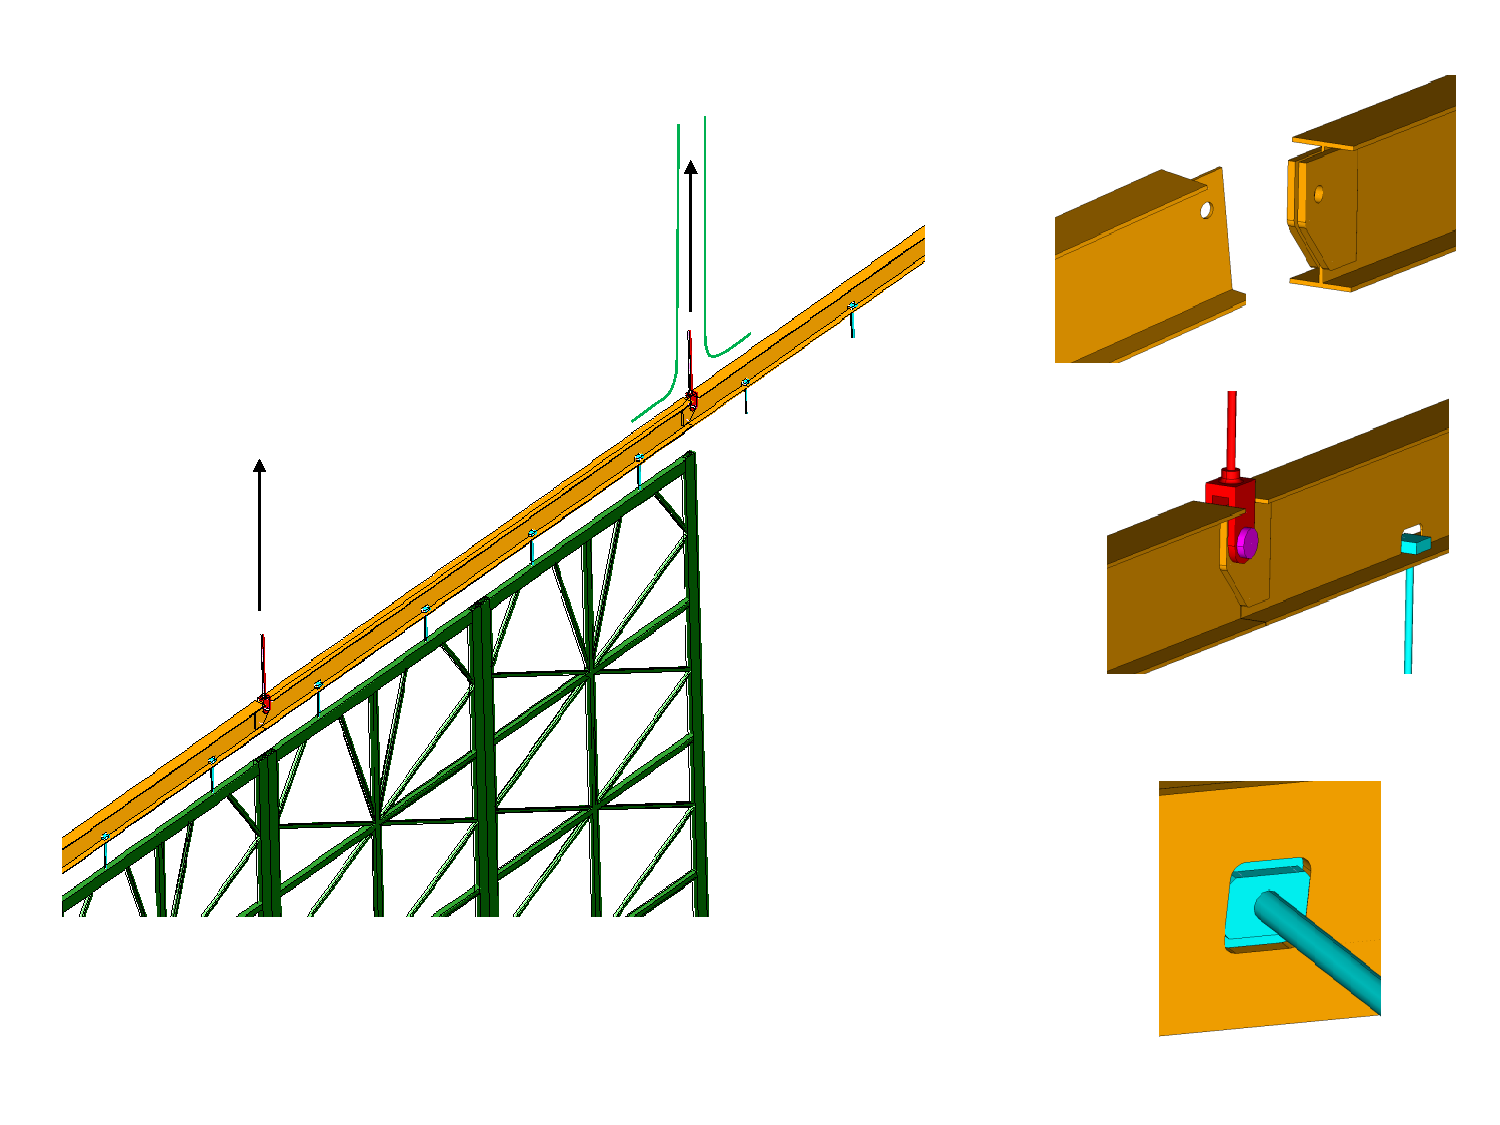
\includegraphics[width=\textwidth]{v5chIC_support-rails}
\end{cdrfigure}

%%%%%%%%%%%%%%%%%%%%%%%%%
\subsection{Discussion of ports in the top of the cryostat}
% (Fowler)}
\label{fd:install:integ:topports}

Each of the APAs will require various electrical services for operation.  This includes bias voltages, power and control lines.  The data will be carried out by signal cables.  The photon detectors mounted inside the APAs will also have cables to carry out their signals.  Inside the cryostat all of these cables will be copper.  
An electronics feedthrough is required at the boundary between the cold LAr volume and the warm ambient above the cryostat.  These feedthroughs will be based on a standard 10-in cryogenic conflat flange mounted on an 8-in tube that will pass through the thickness of the cryostat roof.  Like other LAr detectors, this flange will either have a series of connectors or printed circuit boards with connectors to transition from the cold to warm side.  On the cold side, the cables will be routed from the APAs up to and connected to the cold side of the feedthrough flange.  On the warm side, the cables and data fibers will be routed from the flange to various electronics racks positioned on top of the cryostat.  
Each feedthrough will serve two APAs.  A conceptual layout for the feedthroughs is shown in figure ~\ref{fig:tpc-install-feedthroughs}.  For the upper APAs, the cables will be preinstalled and routed from the cold side of the feedthrough down and along the support rail to the place where they will connect to their corresponding APA.  The feedthrough flanges will be positioned along the length of the APA rows and spaced based on the widths of two APAs or about every 5-m.   For the lower APAs with the electronics near the floor of the cyrostat, the cables will be routed from the cold side of the feedthrough down the side walls of the cryostat.  When the cables are reach the floor they will be routed over to their corresponding APAs.  The lower APA cables will be routed in cable trays supported from the cryostat.  The feedthroughs will be positioned near the outer edges of the cryostat to minimize the cable lengths.  Their spacing will also be approximately every 5-m.  

%\fixme{add a ref to fig}

\begin{cdrfigure}[Feedthroughs]{tpc-install-feedthroughs}{Feedthroughs}
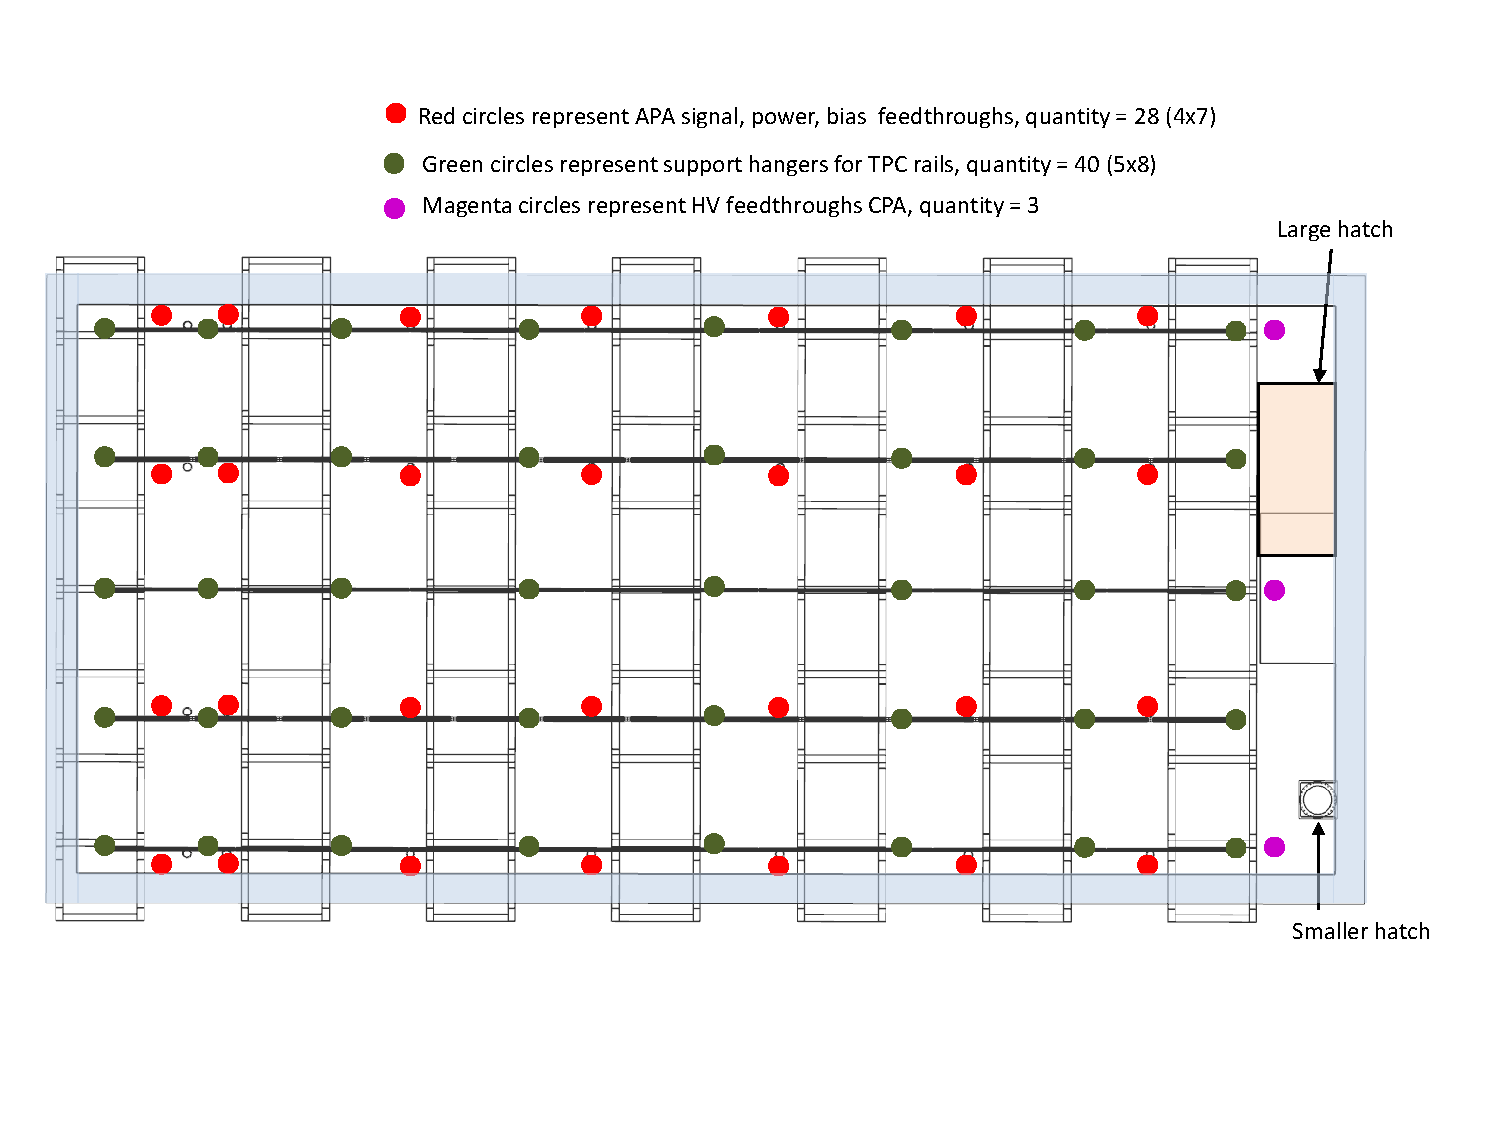
\includegraphics[width=\textwidth]{feedthroughs}
\end{cdrfigure}



%%%%%%%%%%%%%%%%%%%%%%%%%%%%%%%%%%%%%%%%%%%%%%
\section{Installation Equipment - Temporary Equipment}
\label{fd:install:tempeqp}

The below-ground pre-installation activities must be completed prior to the start of TPC installation into the cryostat. These activities include design, procurement and installation of detector-specific 
infrastructure such as man-lifts, lifting fixtures, catwalks, ladders, tools, and so on. The major items include a clean space for the unpacking and preparation of the TPC components, the support rails for the 
TPC panels, the staging platform for joining two panels, installation monorails for moving the panels inside and outside of the cryostat, and a mobile scaffold for providing access to 
the top and middle of stacked TPC panels. 

%%%%%%%%%%%%%%%%%%%%%%%%%
\subsection{Clean Area Outside cryostat}
\label{fd:install:tempeqp:cleanarea}

A clean-area enclosure in the range of class 10,000 (ISO 7 equivalent) will be constructed near the entrance to the cryostat to keep the area around the open hatch isolated. The assembly practices used by 
the MicroBooNe experiment may serve as an example of what is required for a surface detector. The enclosure will have an area for personnel to gown with the appropriate clean-room clothing and safety 
shoes. A large, closable door, next to which the TPC-storage containers can be parked, will allow unloading of the TPC components directly from the container into the clean area. The TPC components 
will be cleaned and protected to a level suitable for installation into the cryostat as part of the TPC production process and will be delivered to the Far Site in clean containers. 

The Double Chooz detector developed a cleanliness plan to ensure that dust contamination did not contribute more than a specified amount to the detector signal. Measurements were made of the activity 
of rock in that experiment’s underground laboratory which was assumed to be the source of airborne dust. Maximum allowable dust concentrations and the clean-room class and cleanliness practices were 
determined such as to meet the requirements for contamination. The Installation and Commissioning group will need to evaluate the dust sources in the LAr-FD detector pit and determine if a similar 
approach to setting the clean room requirements is appropriate. 

%%%%%%%%%%%%%%%%%%%%%%%%%
\subsection{Inside cryostat}
\label{fd:install:tempeqp:inside}

Several items will be installed in the cryostat for use during TPC installation, and removed before the cryostat is filled with argon. 
\begin{itemize}
\item A temporary lighting system inside the cryostat with emergency backup lighting will be in place for TPC installation and removed in sections as the TPC is installed and be completely removed before filling the cryostat with Argon. This lighting system will also be filtered to the appropriate spectrum to protect the photon detection system installed in the APAs.  
\item A ventilation system and air-monitoring sensors with alarms will assure adequate air quality for the personnel working inside the cryostat. The system will also include a high-sensitivity smoke-detection system that is interlocked to the power for all devices inside the cryostat. The blowers and temperature control will be located outside of the cryostat and polyester ducts will be located inside the cryostat to distribute the air properly. 
\item A raised-panel floor to protect the cryostat floor; see Figure~\ref{fig:raised-floor-protect}. The raised-panel floor will have support spacers located between the convolutions in the stainless-steel primary membrane to provide a flat surface for moving equipment around within the cryostat. The pressure limit for the insulation in the floor is 0.5 MPa and the load of the vacuum that will be used to monitor leakage during installation reduces the effective limit to 0.4 MPa. The stock round spacers in the raised-panel floor are 10-cm diameter and would support a load of 310 kg. The load can be increased by adding larger-diameter plates under the standard spacers. Since the raised floor is modular, it can be removed in sections as the TPC installation progresses. A perforated pipe manifold will be located on the cryostat floor to distribute the argon during the gas piston purge and during liquid recirculation. Depending on the details of the membrane cryostat corrugation height, the distribution piping may fit under the temporary floor or be installed in sections as the floor is removed. 
\item Tooling for APA and CPA panels including fixtures to insert the lower APA and CPA panels. The top and bottom TPC panels of a stacked pair will be moved into the cryostat separately and connected together below the cryostat equipment hatch. A lower panel holding fixture will temporarily hold the bottom APA and CPA panels when they are inserted into the cryostat. See Figure~\ref{fig:panels-lowered-hatch}. 
\item Two fixed scaffolds with integral stair towers will be installed temporarily inside the cryostat. One tower will be located in the work area of the large hatches. This tower will provide access for personnel to make the connections between stacked panels and to connect stacked panels to the installation rail inside the cryostat. The second fixed tower will be located near the smaller hatch and will provide a second route of egress from the cryostat. 
\item A rolling scaffold with an integral stair tower will allow personnel to access the top of the stacked panel after they are in the final position. The rolling scaffold will be moved around the cryostat floor as the TPC installation progresses. 
\end{itemize}

\begin{cdrfigure}[Raised-panel floor to protect the cryostat's primary membrane]{raised-floor-protect}{Raised-panel floor to protect the cryostat's primary membrane}
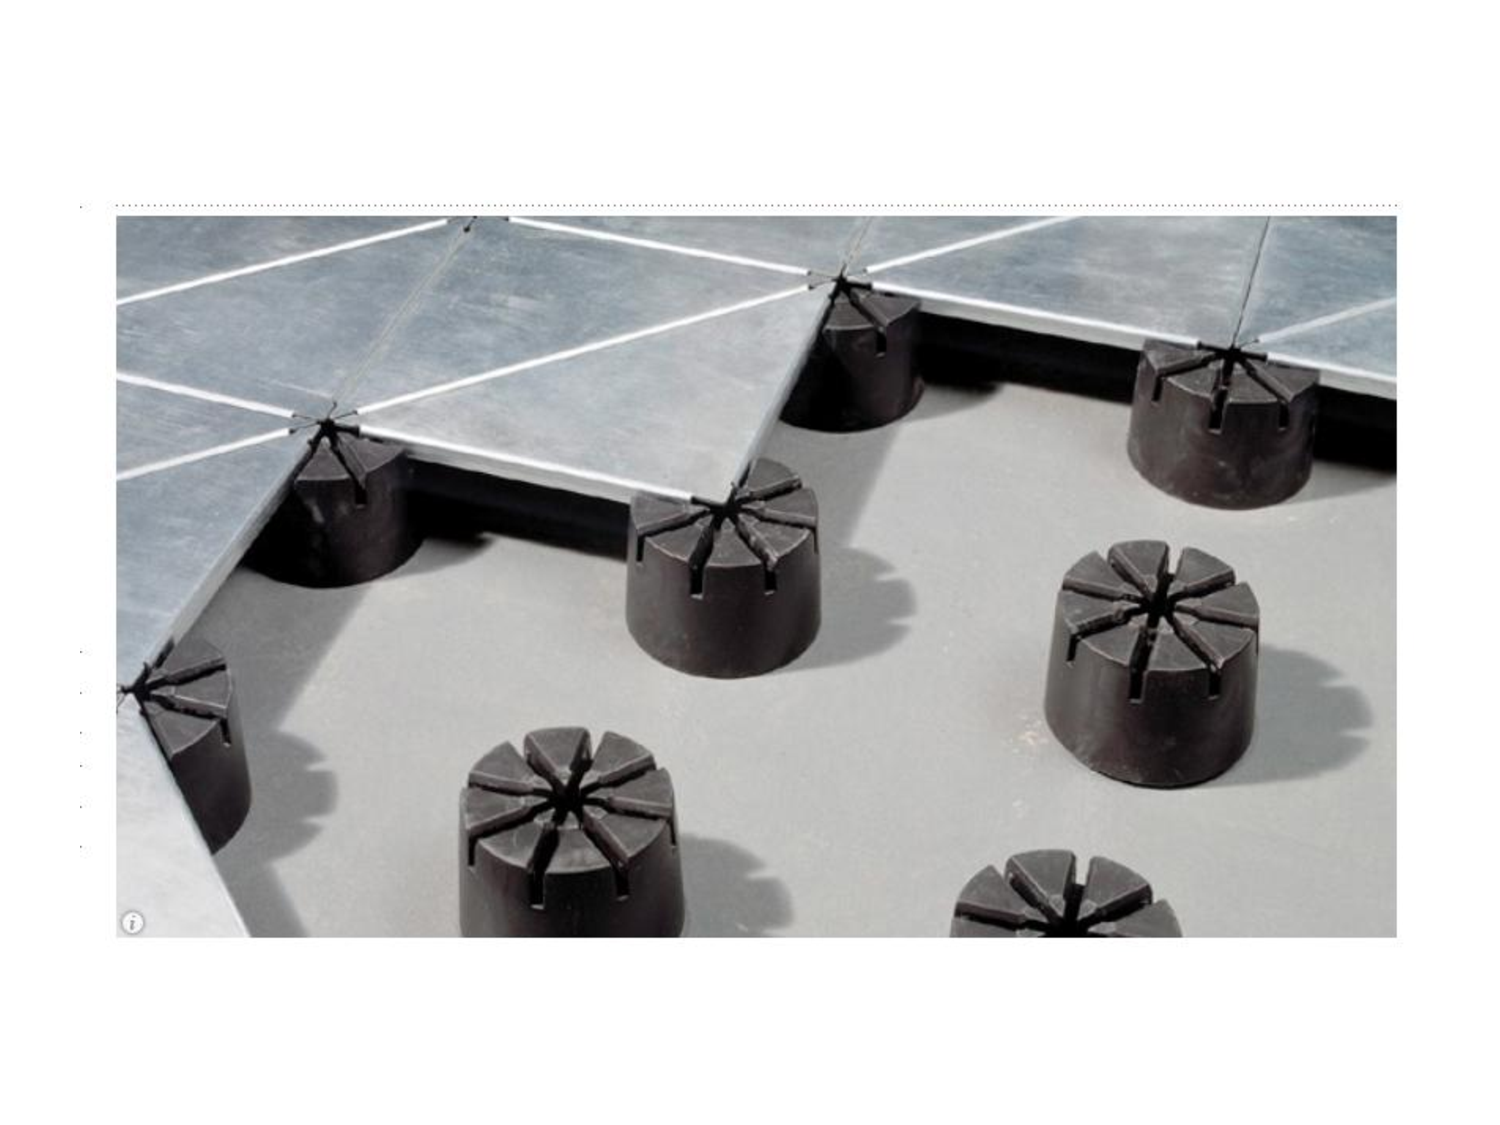
\includegraphics[width=0.8\textwidth]{v5chIC_raised_floor}
\end{cdrfigure}


%%%%%%%%%%%%%%%%%%%%%%%%%
\subsection{Full-scale Mockup}
\label{fd:install:tempeqp:fsmockup}

A full-height mock TPC section will be constructed as part of an installation prototype in a suitable location at Fermilab, e.g. the Wideband lab or D-zero assembly hall. See Figure 12 \fixme{need to find}. The installation 
equipment prototype is intended to test and verify the key elements of the equipment and the process for TPC installation and to serve as a training tool for personnel who will perform the TPC installation. The initial testing of the equipment at Fermilab will be used to verify or refine the installation concepts. 
Complete testing of the final equipment and operations will occur at Fermilab before the installation equipment is moved to the Far Site. 

This prototype will include APA and CPA rail supports and cable routing features. Multiple mock-ups of APA and CPA stacked panels will be installed. The APAs will include all mechanical mounting points and 
some electrical connections such as optical-fiber readout cables and power cables. Prototype versions of the special equipment required for TPC installation will be used, including the trolley, lower-panel 
staging platform, and a rolling-cart scaffolding. Scaffolding elements will be rented and the scaffolding will be erected by a contract or as part of a training program. 

Initial tests, where appropriate, will be performed at a low elevation. For example, the installation trolley 
and rail segment will be tested at a low elevation with a dummy weight. After successful demonstration of the features in this position, the components will be moved to a high elevation for testing with full-
size mock-up panels. 

\begin{cdrfigure}[Installation equipment mockup to be built and tested]{installation-equipment-prototype}{An Installation equipment mockup of a TPC section, in blue, will be built and tested in a Fermilab assembly building like the Wideband lab shown here}
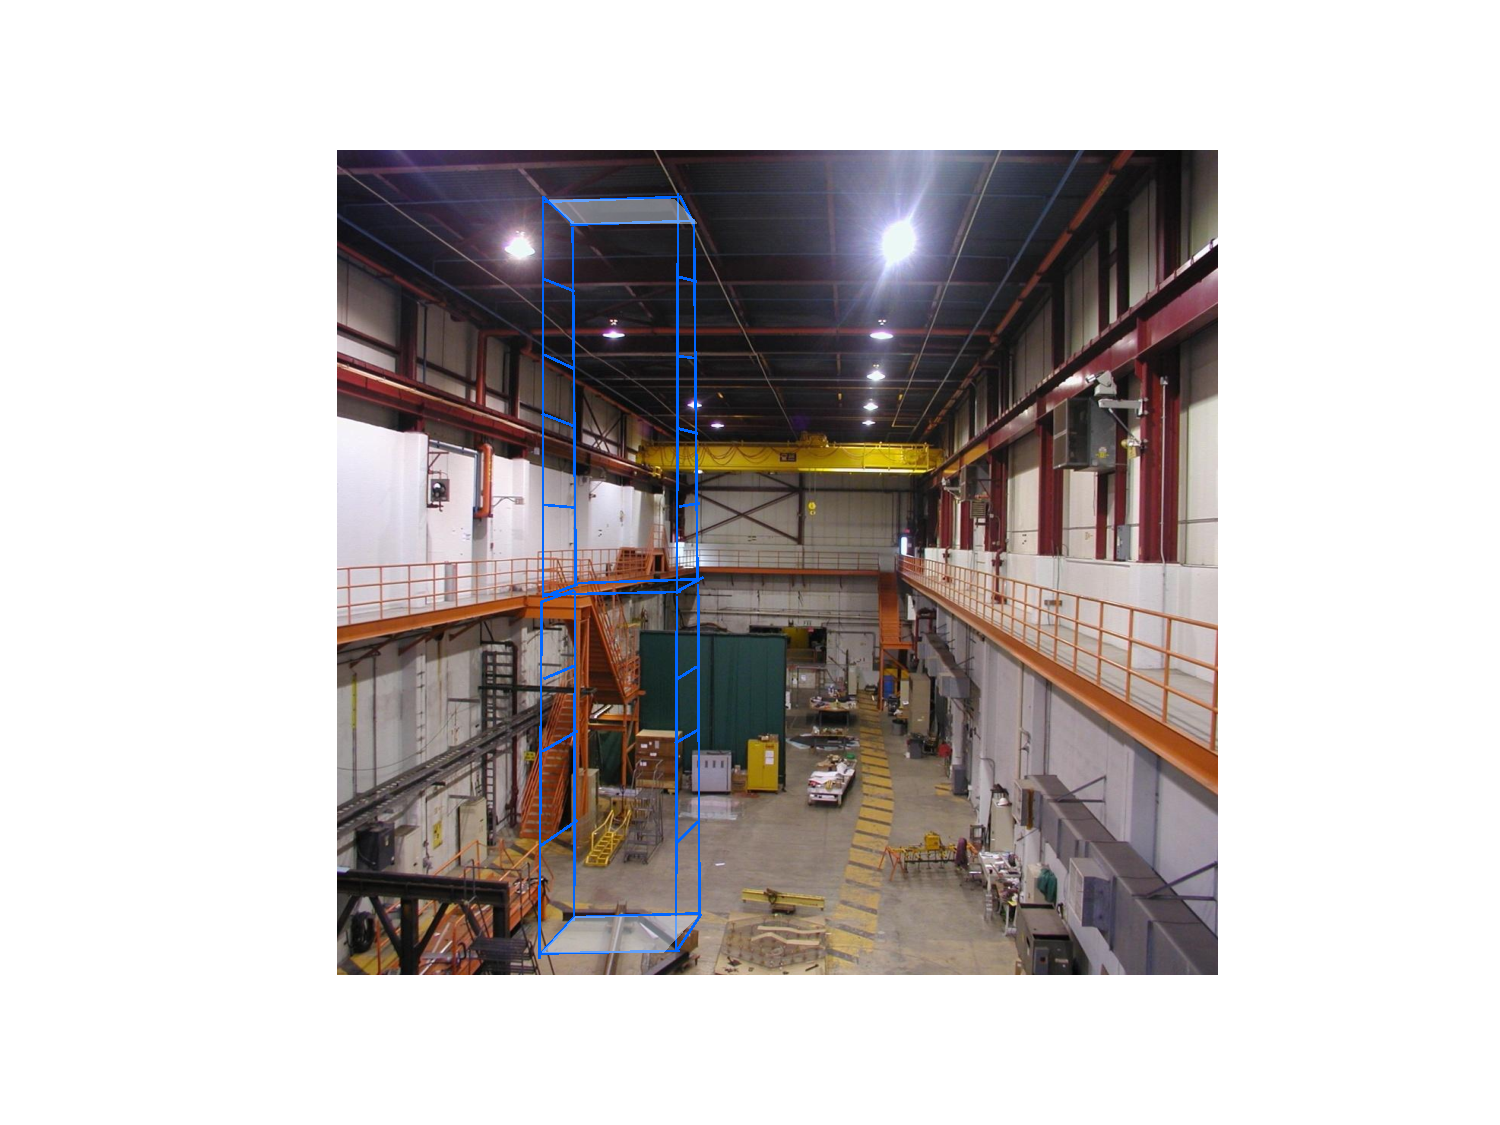
\includegraphics[width=\textwidth]{v5chIC_installation-equipment-prototype}
\end{cdrfigure}


%%%%%%%%%%%%%%%%%%%%%%%%%
\subsection{Surface at SURF}
\label{fd:install:tempeqp:surfsurface}

Materials for the TPC will be transported down the Ross shaft from the surface to the 4850-ft level.  It is planned that most of the material for the TPC can be sized such that it will fit inside and be transported by the cages in the Ross shaft.  The APAs are too large and will be slung underneath the cage inside a specially designed container.  Space and equipment will be required to move the standard and special container into the cages and attach the slung loads underneath the cage.  

%%%%%%%%%%%%%%%%%%%%%%%%%%%%%%%%%%%%%%%%%%%%%%
\section{Far Site Installation}
\label{fd:install:fsinstall}

%%%%%%%%%%%%%%%%%%%%%%%%%
\subsection{Far site activities overview}
% (Howell)}
\label{fd:install:fsactivities}

Local storage in the SURF region will be required because Detector installation is much shorter duration than the detector fabrication/assembly time. The local storage facility will also be used for checkout and 
testing of Detector components. The installation space in the cavern is very limited and so material will be moved from the local storage to the cavern at the rate of installation. Prior to installation, a clean area 
will need to be setup in the cavern just outside of the cryostat (Figure~\ref{fig:clean_area}). After the clean area is configured, temporary installation equipment will be installed in the first cryostat. TPC installation will proceed in the 
first cryostat and as temporary equipment is removed from the first cryostat it will be installed into the second cryostat to prepare for installing the second TPC.

\begin{cdrfigure}[Underground clean area arrangement]{clean_area}{Underground clean area arrangement}
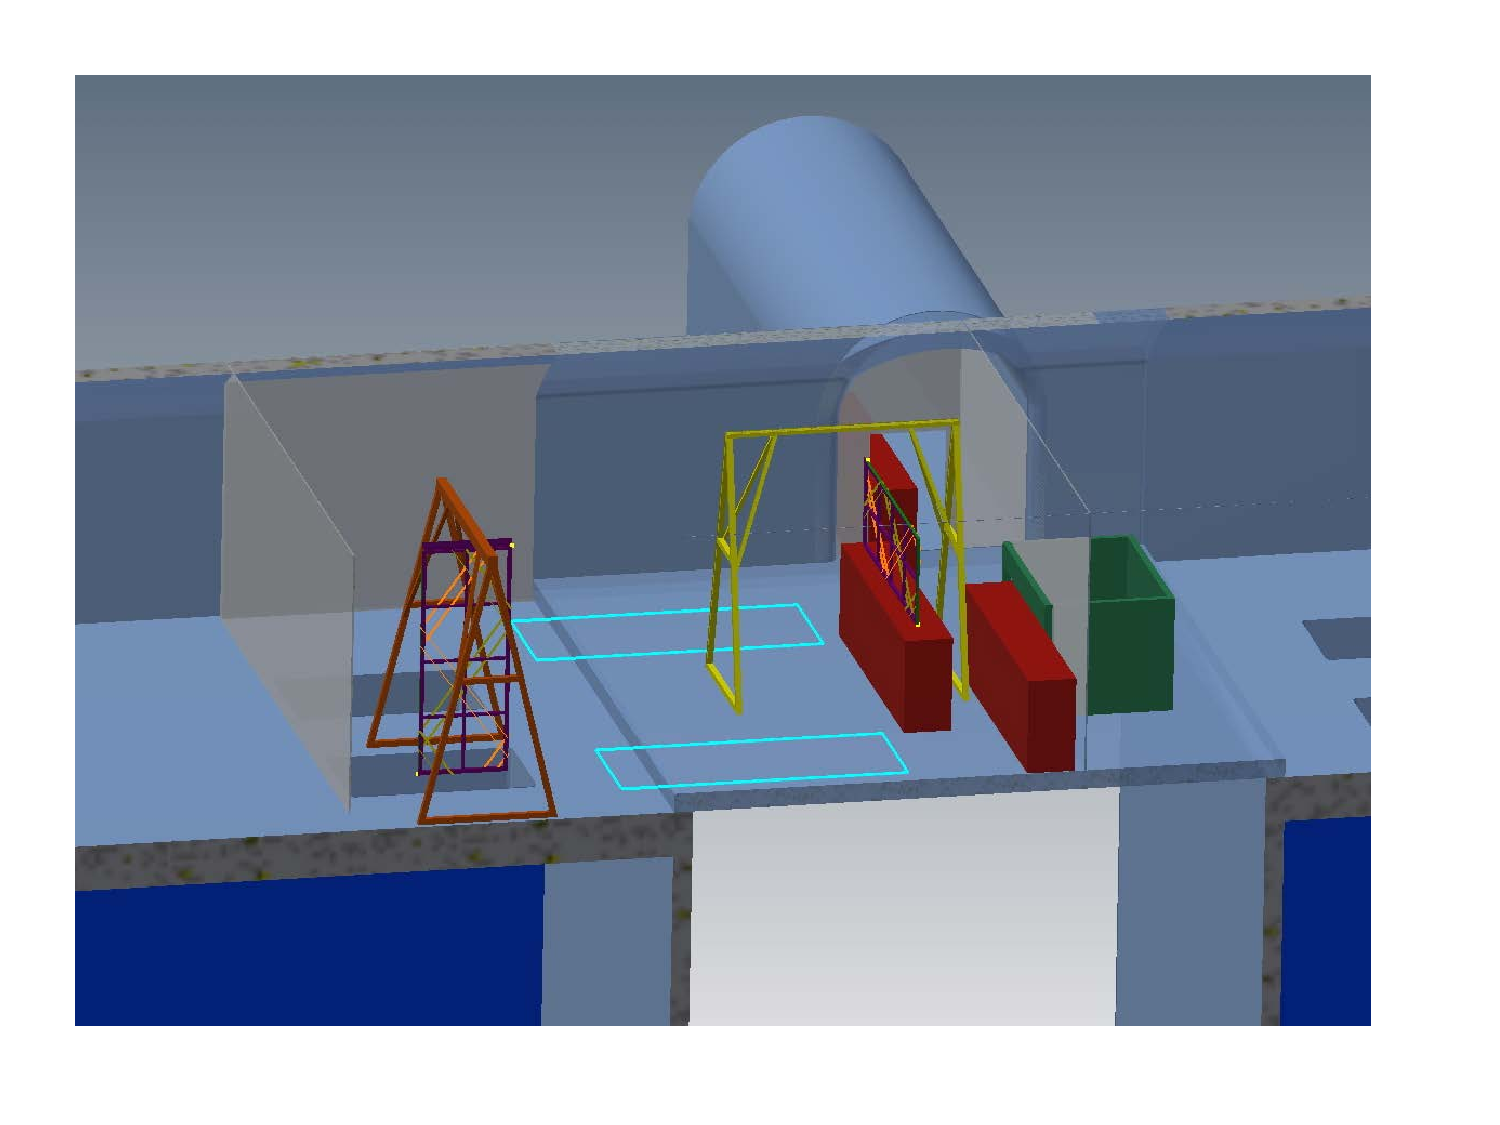
\includegraphics[width=0.8\textwidth]{underground_clean_area_arrangement}
\end{cdrfigure}


The following list of detector components and systems will be installed in the Detector Hall and cryostats: 

\begin{itemize}
\item Relay Racks with rack protection (28 on each cryostat plus a few in the control room) 
\item Cable trays and power distribution to racks from power panels provided by CF 
\item Cable inside and outside of the cryostat including cable feedthrough flanges 
\item DAQ crates and power supplies in the relay racks 
\item The 52 APAs per cryostat with integrated photon detectors 
\item Three times the equivalent active area of the APAs of CPAs per cryostat 
\item Cryogenic instrumentation not installed by the cryostat construction vendor (e.g. purity monitors) 
\item Temporary ventilation, lighting and access equipment 
\item Note: Support rails and hangers are installed during cryostat construction 
\end{itemize}

\begin{cdrfigure}[TPC panels installed in cryostats]{tpc-panels-in-cryostat}{TPC panels installed in cryostats}
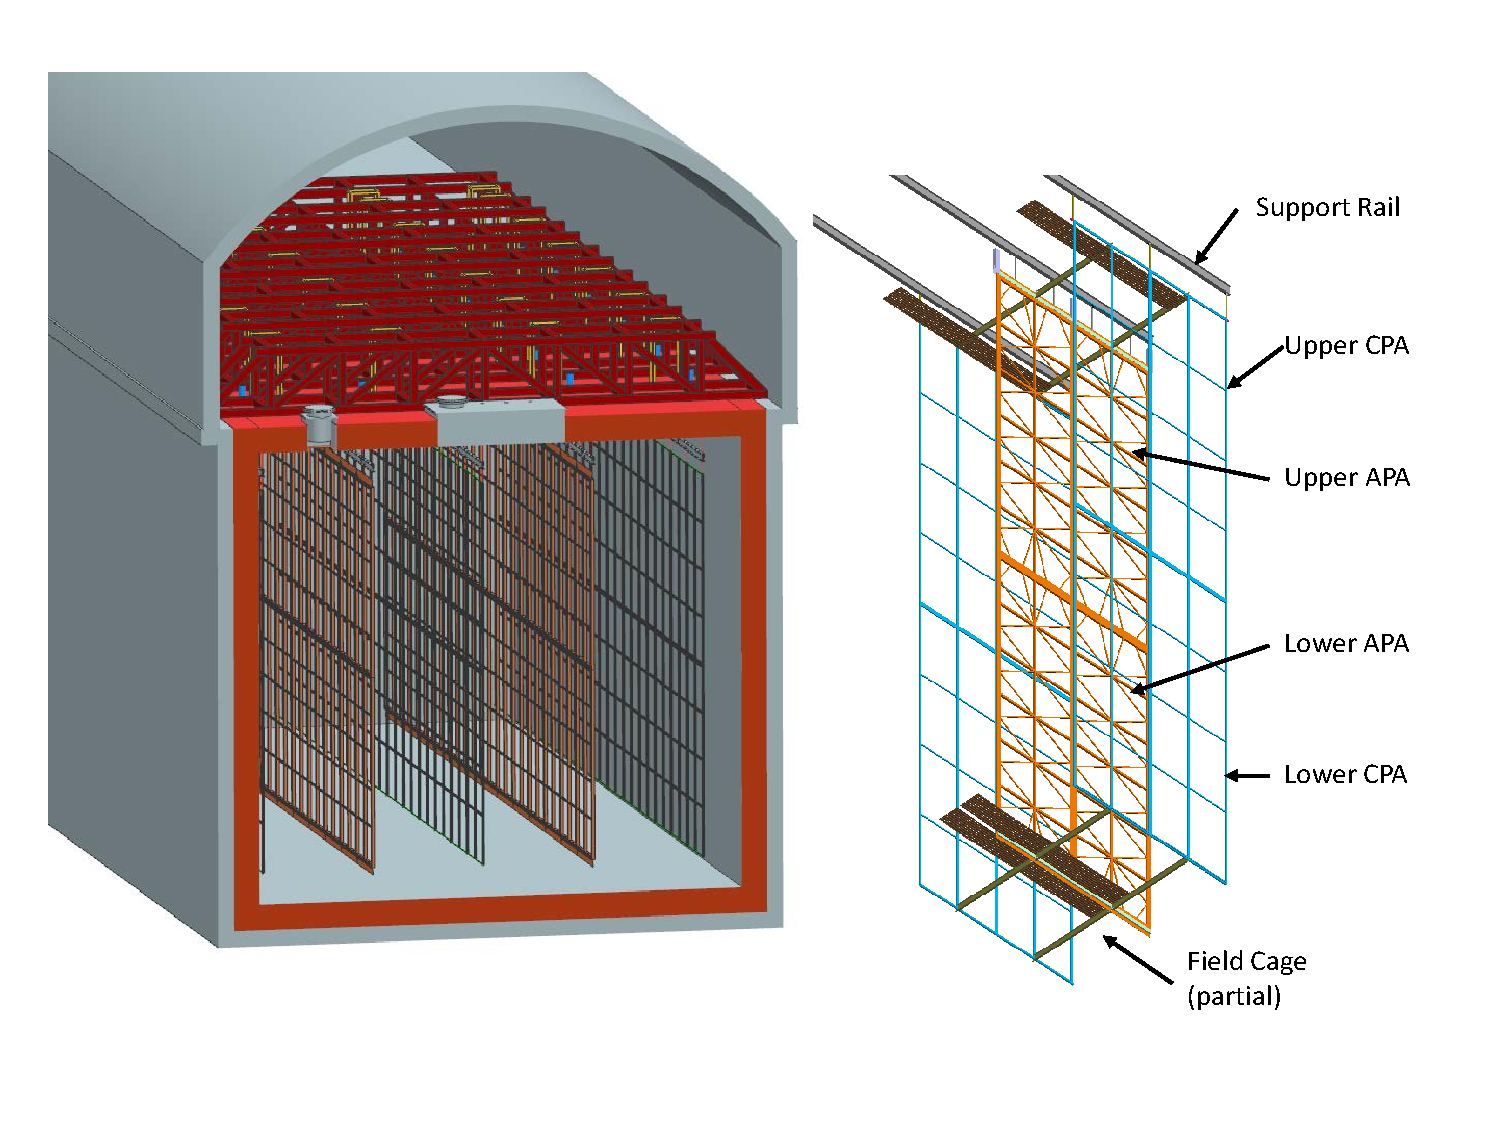
\includegraphics[width=0.8\textwidth]{TPC_installed}
\end{cdrfigure}

%%%%%%%%%%%%%%%%%%%%%%%
\subsection{Detector material storage /testing above ground}
% (Howell)}
\label{fd:install:fsinstall:mat:storage}

Detector components will be delivered to the Far Site over a period of many months and will need to be stored in a storage facility. This will allow the supply of material to be maintained ready for installation. The facility will 
also be used for testing and checkout of the APA after the shipment from the manufacturing sites. Depending on the APA design and assembly flow the storage/testing facility may also be used for installation of the photon 
detectors and/or the installation of cold electronics on to the APAs.  A facility for this purpose will be identified in the SURF region and arrangements will be made for its use during LAr-FD construction. Each system group is 
responsible for delivery of its components to the storage/testing facility. The Installation and Commissioning group will provide the management and labor resources for inventory control, material handling and transport from the off-site facility to the Detector Cavern. 


The majority of the storage/testing facility space will be required for storage and testing of APAs. The APA will be shipped from the APA assembly sites to the SURF area in semitrailers or 40 ft long cargo containers. The APAs 
will be held in a vertical plane in a rack with one rack of about 10 APAs fitting in each trailer or container. It will expected that the racks can be removed from shipping container (Figure~\ref{fig:apa_ship}) and the APAs can remain in the racks as they are 
moved and stored.  The racks will have an approximate footprint of 8' x 22'. About 12 such racks will be needed for each cryostat approximately with 2500 ft2 required for all APA storage. The CPA and field cages material can be packed more compactly and will required additional space of approximately 2,500 square feet.

\begin{cdrfigure}[Concept for APA shipping containers]{apa_ship}{Concept for APA shipping containers}
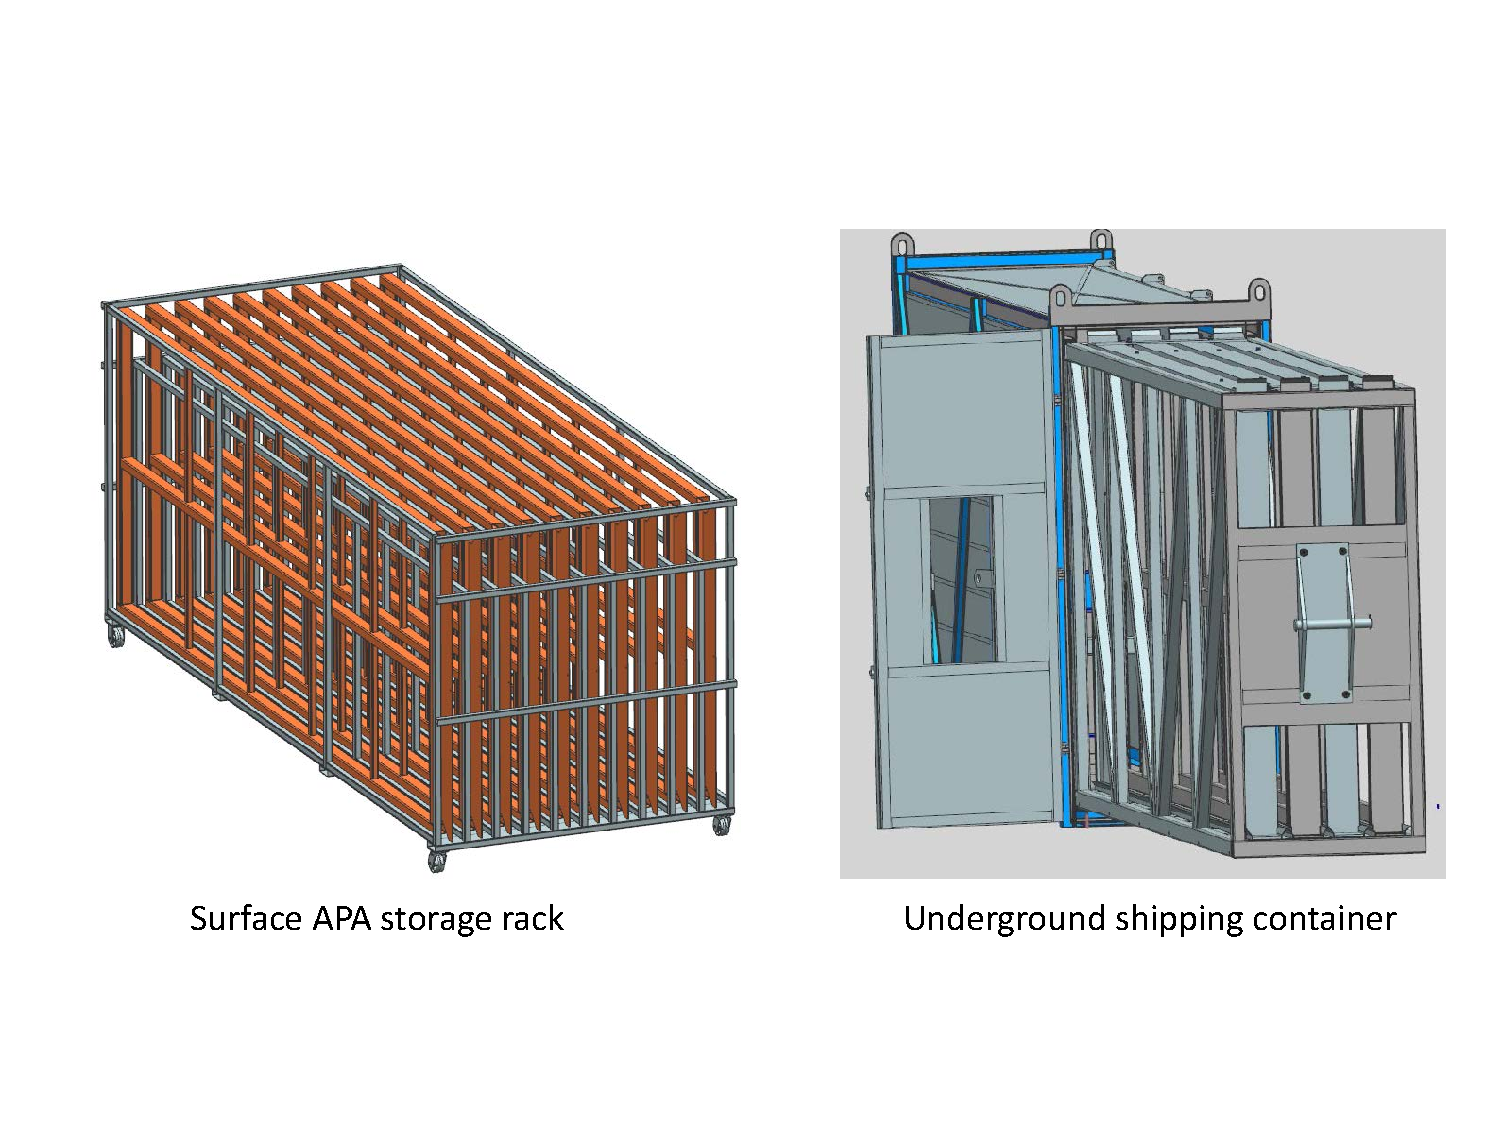
\includegraphics[width=0.8\textwidth]{apa_ship}
\end{cdrfigure}


The facility will also be used for checkout and testing of the APAs after the long distance shipment from the assembly sites. In addition, the facility may also be used for some assembly tasks such as installing the photon 
detectors. Since the APAs will be exposed during these operations, the work lighting will have UV filters installed and air recirculation units will be used to maintain a clean area in the range of class 10,000 (ISO 7 equivalent). 
There will be a few of stations for check out , inspection and transfer of the APAs. Approximately 5000 ft2 will be required for these functions with a clear height of approximately 20ft to allow the APAs to be lifted out of storage 
racks and stations. With a modest weight less than 1/2 ton, a free standing workstation crane would be sufficient for lifting the APAs.

The storage/testing facility should be located with a one hour drive of SURF. The facility could be in Rapid City or in the area close to SURF. The final choice of location will be a compromise of many factors including available 
lease space, workforce availability and cost.

%%%%%%%%%%%%%%%%%%%%%%
\subsection{Material movement to cavern}
% (Howell)}
\label{fd:install:fsinstall:mat:movement}

Material will be transferred from the storage facility to the Detector Hall for installation, as required to sustain the installation rate. The Ross shaft will be used to move material underground. It is possible that the CPA and field cage 
materials can be sized such that they will fit into the Ross shaft cage. However the APAs are two long and must be slung underneath the Ross cage. 

A conceptual design for a special APA transportation container has been developed that will hold 4 APAs in horizontal and vertical orientations for movement in the Ross shaft. The 60" distance between the rails of the 
Ross shaft limits the width of objects that can be lowered down the shaft. 

The Ross shaft lift has provisions to attach long objects to the bottom of the cage. The APA in a special container will descend the shaft in a vertical orientation 
(the same orientation as they will be installed), be rotated to a horizontal orientation as they are extracted from the shaft, then moved along the access drift on a cart to the cavern. The APA transportation container consists of 
an internal rack that can be extracted from the outer container thus avoiding moving the outer container into the clean area used for installation. The internal rack will be used to hold the APA in the installation area until they 
are installed. Empty racks will be returned to the warehouse for reloading in the transportation container. Figure~\ref{fig:warehouse_arrangement} shows the warehouse arrangement.

\begin{cdrfigure}[Warehouse arrangement]{warehouse_arrangement}{Warehouse arrangement}
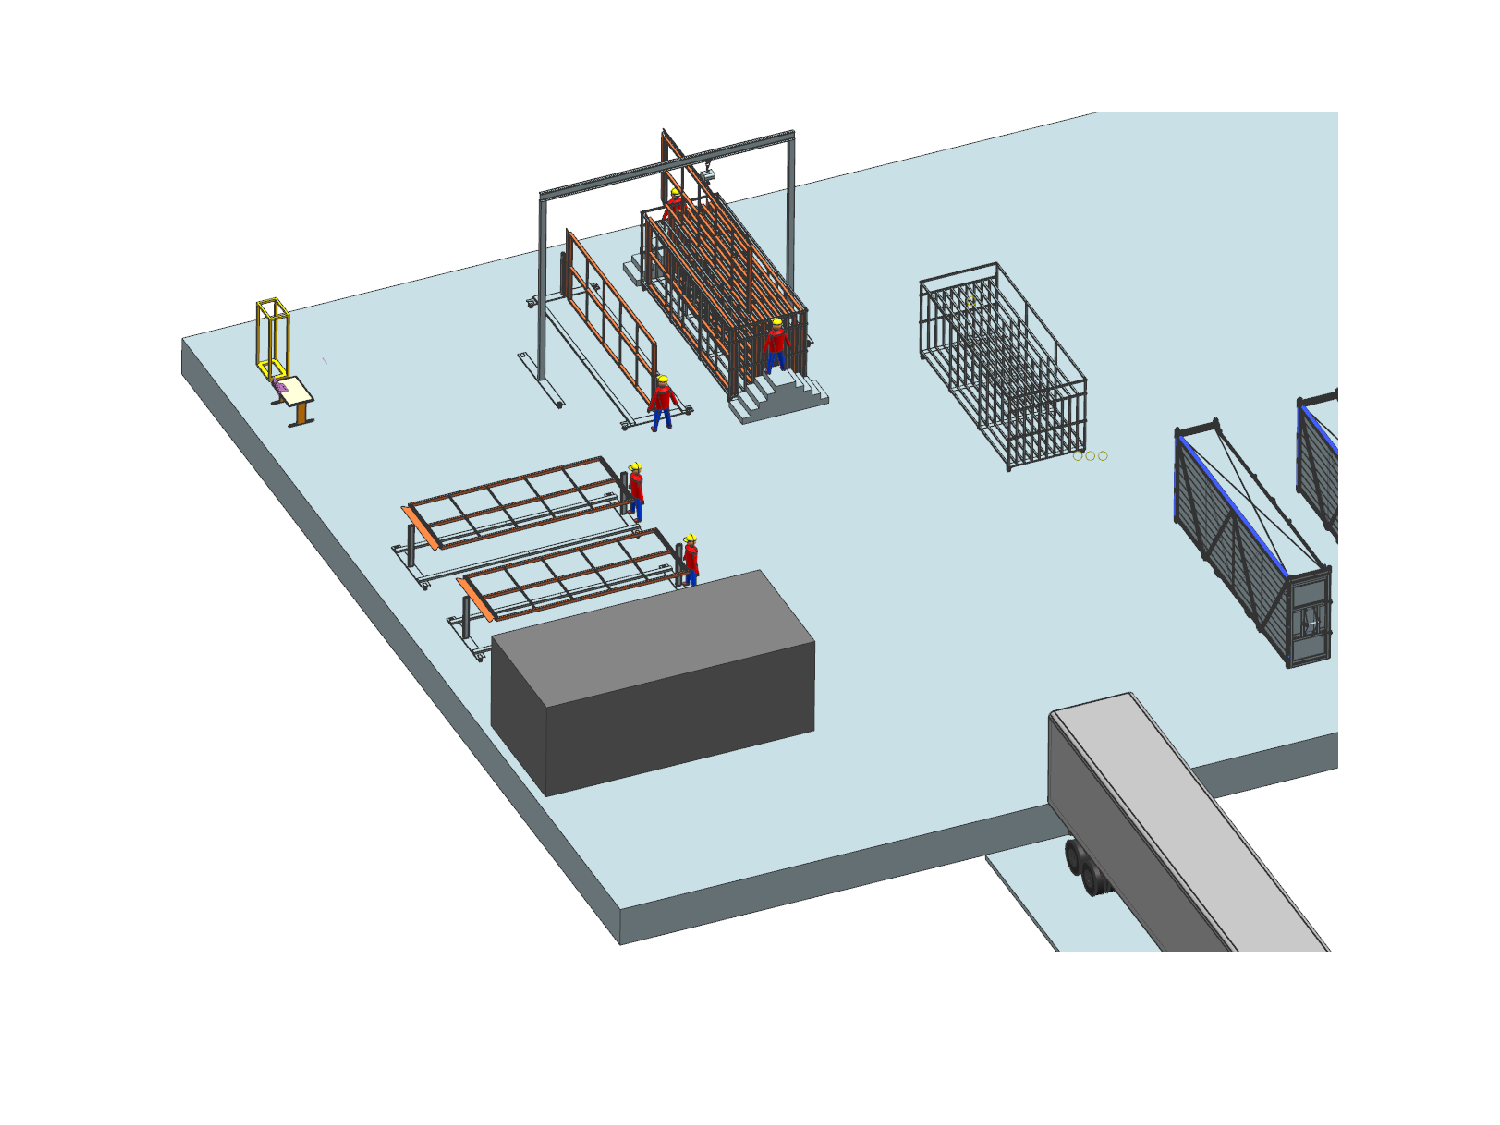
\includegraphics[width=\textwidth]{warehouse_arrangement}
\end{cdrfigure}


%%%%%%%%%%%%%%%%%%%%%%
% We decided that this was covered in the other sections and will leave it out
%\subsection{Setup and equipment arrangement in clean area (Fowler)}
%\label{fd:install:fsinstall:setup:cleanarea}

%\fixme{Need content! And move figure here if we get content}

%%%%%%%%%%%%%%%%%%%%%%
\subsection{TPC installation details}
% of steps) (Fowler)}
\label{fd:install:fsinstall:tpc:install:steps}

Each APA and CPA panel will be carefully tested after transport into the clean area at the septum and before installation into one of the cryostats. Immediately after a panel is installed it will be rechecked. Throughout the 
installation period it will be checked periodically. The serial stacking of the APA panels along the rails means that removing and replacing one of the early panels in the row after several others are installed would be 
very costly in effort and time. Therefore, to minimize the risk of damage, as much work around already-installed panels as possible will be completed before proceeding with further panels. 

The installation sequence is planned to proceed as follows: 
\begin{enumerate}
\item Install the monorail or crane in the staging area outside the cryostat, near the equipment hatch. 
\item Install the relay racks on the top of the cryostat and load with the DAQ and power-supply crates. 
\item Dress cables from the DAQ on the top of the cryostat to remote racks. 
\item Construct the clean-room vestibule outside the cryostat hatch. 
\item Install the raised-panel floor inside the cryostat. 
\item Insert and assemble the stair tower and mobile scaffold. 
\item Install the staging platform inside the cryostat.
\item Install protection on (or remove) existing cryogenics instrumentation in the cryostat. 
\item Install the cryostat feedthroughs and dress cables inside the cryostat along the support beams. 
\item Begin regular transport of TPC panels in shipping boxes into the cavern. 
\item Install TPC panels: 
\begin{enumerate}
\item Install the two outer CPA wall assemblies.  This is done by building the CPA one horizontal strip at a time.  Once a strip is assembled, it is lifted and another strip is attached below until the entire height is reached.  It is unclear at this point what length of strip is feasible to install at once.  This length is expected to correspond to some multiple of the distance between the support hangers.  
\item Install the center CPA.
\item Install the end wall field cage between the two outer CPAs and the existing center row. 
\item Begin the installation of the first row of APAs.
\item Lower the first APA with the electronics toward the bottom of the cryostat and fix in the transfer fixture.
\item Lower the second APA with the electronics toward the top of the cryostat.
\item Mechanically join the two APAs in the center.  
\item Lift the connected pair of APAs onto the support rail.
\item Move the stacked pair of APAs down the rail to their installed position.  
\item Link the stacked pair to the adjacent stacked pair of APAs.
\item Connect power and signal cables. 
\item Test each APA wire for expected electronics noise. Spot-check electronics noise while cryogenics equipment is operating. 
\item Connect field cage in sections as the APA and CPA installation progresses at the top. 
\item Perform electrical test on CPAs and field cage. 
\item Remove temporary floor sections as the TPC installation progresses. 
\item When a row of APAs is completed, install any argon distribution piping under the APAs and associated CPAs.
\item Install the lower field cage panels for this row of APAs.
\item Install the end field cage for this row of APAs and associated CPAs.
\item Move the mobile scaffold to the second row of APAs.
\item Move installation scaffold and transfer fixture to the second installation hatch. 
\item Repeat the APA installation on the second row of APAs.
\end{enumerate}
\item Complete the end field cage.
\item Remove the transfer fixture, moving platform and stair tower from the cryostat. 
\item Temporarily seal the cryostat and test all channels for expected electronics noise. 
\item Seal the access hatch. 
\item Perform final test of all channels for expected electronics noise.
 \end{enumerate}
 
In general, APAs and CPAs will be installed in order starting with the panels furthest from the hatch side of the cryostat and progressing back towards the hatch. The field cage will be installed in stages as the installation 
of APA and CPA panels progresses at the top to utilize the mobile access platform. The only requirement for survey or alignment is to maintain the edges of a row of APA panels to 3-mm alignment along each beam. A laser guide or optical transit in combination with the 
adjustment features of the support rods will be used to establish the alignment. After the stacked panel is attached to the support rods the electrical connections will be made to cables that were already dressed to the support rail 
and electrical testing will begin. Periodic electrical testing will continue to assure that nothing gets damaged during the additional work around the installed panel. 

After the CPAs have been installed, the APA installation will be performed in three stages, each in a separate location; the locations, or zones, are shown in Figure~\ref{fig:tpc-install-workzones}. First, in the clean room vestibule, a crew will move the APA panels from storage 
racks, rotate to the vertical position and move them into the cryostat. Secondly, in the panel-staging area immediately below the equipment hatch of the cryostat, a second crew will transfer the lower APA panels from the 
crane to the staging platform, connect the upper and lower panels together. After connection, a motorized trolley will move the stacked panels from the hatch area to their final position. Since the duty cycle of the trolley is rather low, the trolley could be battery-powered to 
avoid the need for cable festooning. The trolley initially moves along a rail until it reaches the end where the stacked panel will be permanently mounted. A third 
crew will reposition the movable scaffolding and use the scaffold to make the mechanical and electrical connections at the top for each APA. The rails inside and outside 
the cryostat will each have motorized trolleys so that work can be conducted by all three crews in parallel. The steady-state rate for installation, given this work plan and a single-shift schedule, is estimated to be two stacked panels per day. 

\begin{cdrfigure}[The three main work zones for TPC Installation]{tpc-install-workzones}{The three main work zones for TPC Installation. TPC components are lowered into the cryostat in zone 1. TPC components are connected together in zone 2, 
transferred to the support rails and then rolled into final position (zone 3).}
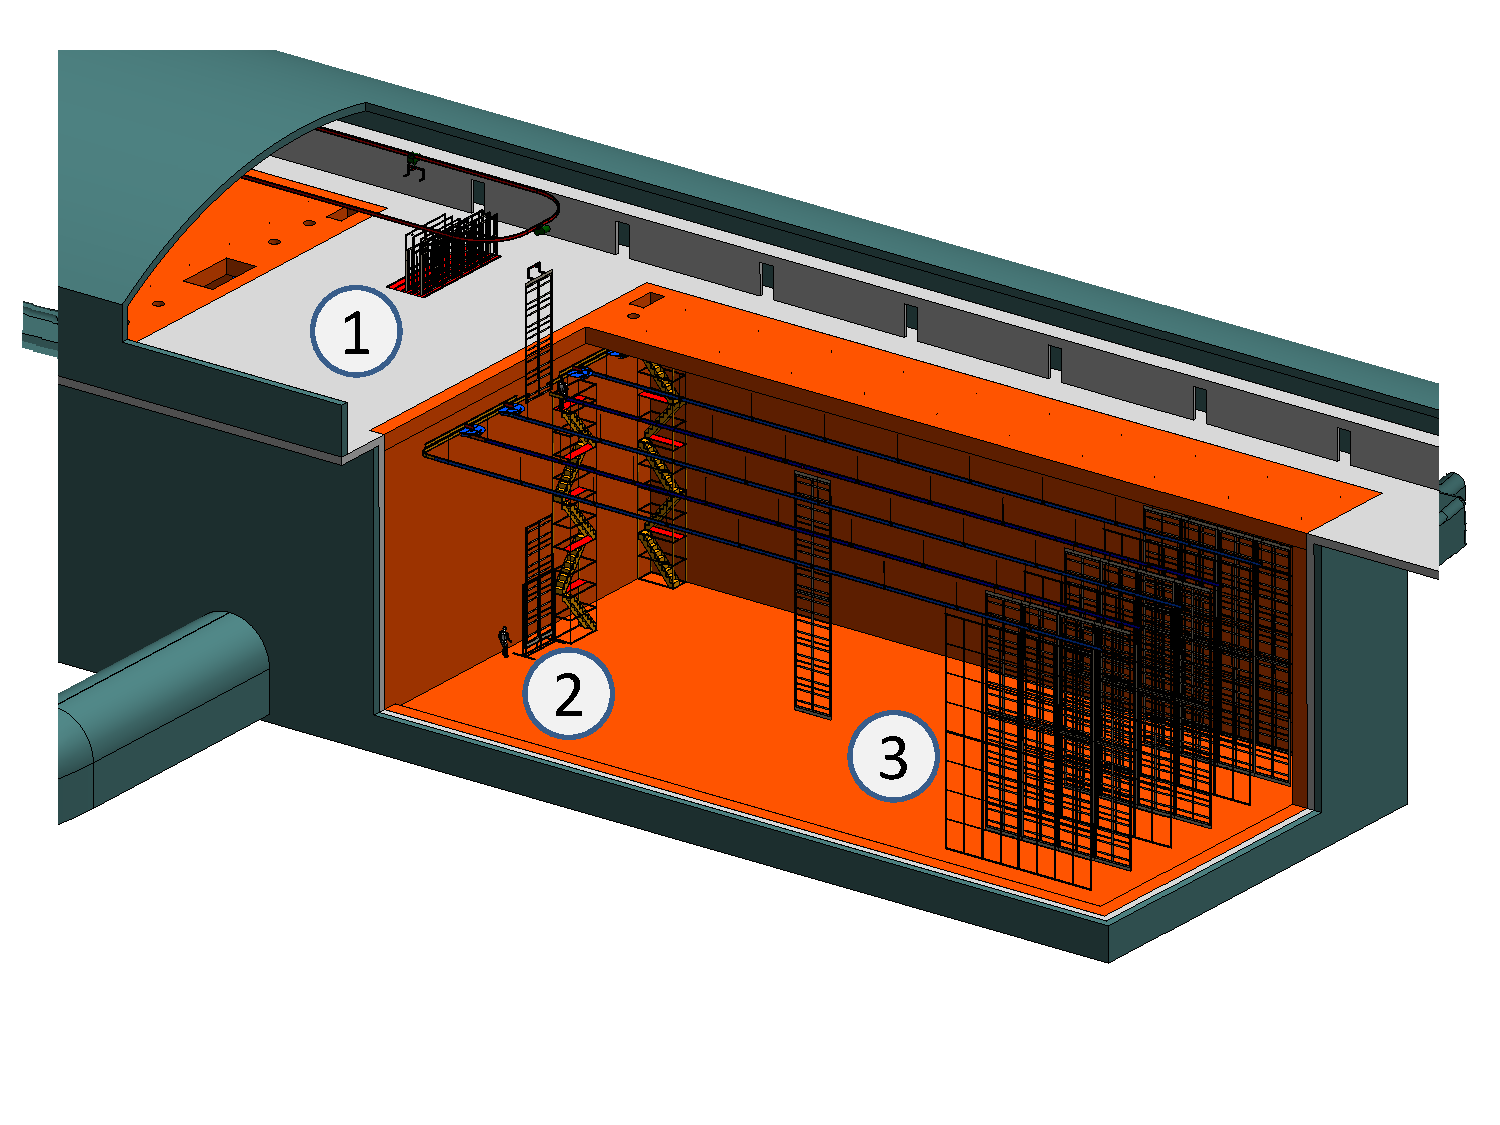
\includegraphics[width=\textwidth]{v5chIC_work-zones}
\end{cdrfigure}

Signal and power cables will be installed from the cryostat feedthrough ports next to the APA support rods, shown in Figure~\ref{fig:tpc-install-feedthroughs}, along the rails to the point where the connection to the APAs will be made. The cables will be 
preplaced and tested before APA installation begins.  Editor’s Note: Figure~\ref{fig:tpc-install-feedthroughs} is for a 17-kton fiducial mass cryostat. The 5-kton cryostat is shorter and has fewer rows.  


The detector installation system is also responsible for developing and implementing the procedure for monitoring the integrity of the membrane-cryostat primary liner during installation. The space between the 
primary liner and the secondary liner will be held under vacuum during installation. The vacuum level will be automatically monitored and will alarm if any leaks develop in the primary membrane during TPC installation

%%%%%%%%%%%%%%%%%%%%%%%%%%%%%%%%%%%%%%%%%%%%%%
\section{Training}
% (Howell)}
\label{fd:install:training}

Installation and Commissioning will be responsible for the personnel, equipment and procedures for providing Detector Hall access controls after cryostat construction is complete. Members of the installation crew will be 
trained on specific installation tasks and must pass a qualification test. The training will use mock-up APAs constructed for the installation equipment prototype. The training program will be developed in collaboration with Fermilab and SURF ES\&H personnel. 

Installation and Commissioning will provide all of the general tools and equipment needed to support the personnel in their installation work. It will include hand tools, power tools, material-handling equipment, ladders, 
lifts, electrical meters and personal protective equipment (PPE). The detector system groups will provide any special equipment to check out or debug the power and read-out chain of the detectors. The detector groups will also provide system experts at the far site to check out the detector systems before and after installation. 

%%%%%%%%%%%%%%%%%%%%%%%%%%%%%%%%%%%%%%%%%%%%%%
\section{Far Detector commissioning}
\label{fd:install:commissioning}

The detector installation and commissioning activities will be staged such that both TPCs can be tested cold while one cryostat still remains available as a potential storage vessel in case a repair is needed. The LAr in one cryostat can be transferred to the other and back again, if necessary, to allow access for a repair. Once both TPCs are known to work properly at LAr temperature, the second fill will take place. 

Commissioning Sequence

The commissioning sequence, illustrated in Figure~\ref{fig:tpc-install-commissioning-seq}, will start with the installation of the TPC into cryostat 1 (installed on the north side). During this time, the leak testing and cleaning of cryostat 2 will be completed and, 
where possible, the setup for TPC installation will begin. After the TPC is completely installed in cryostat 1, its purge and cool-down can begin. These processes are described in Section ?. Filling the cryostat with room-
temperature gaseous Ar, injected from the bottom in order to displace the air upward through the top ports. 

Following the purge and cool-down, the LAr fill of cryostat 1 will take approximately two months, assuming continuous LAr deliveries. LAr purification will begin when the liquid level is high enough to start the recirculation 
pumps. The commissioning of the cryogenics system can also begin at this point, but its full commissioning will require a fully loaded cryostat. In-vessel purity monitors will operate during this time. 

When the cryostat is full with LAr, the TPC will undergo testing for approximately one month to establish that the TPC will be able to achieve the tracking requirements and to confirm that no further access will be needed to the 
cryostat and TPC. Additional testing will occur after the other cryostat is filled and is thus no longer available as a storage vessel. 

\fixme{Find old figure and use it}

\begin{cdrfigure}[Startup and Commissioning Sequence]{tpc-install-commissioning-seq}{Startup and Commissioning Sequence}
%  \includegraphics[width=0\textwidth]{file}
\end{cdrfigure}


Installation of the TPC in cryostat 2 will begin during the LAr fill of cryostat 1. After TPC installation and electronics testing, the purging and cooling for cryostat 2 can proceed. The LAr from cryostat 1 will be 
transferred to cryostat 2, and once it is full, its TPC will undergo a month of initial testing. During this time, cryostat 1 will be maintained cold via continuous circulation of gaseous Ar. After it is established that no further access will be required, cryostat 1 will be refilled with LAr and begin a five-month commissioning period. Testing during the commissioning period will demonstrate that the detector performance parameters for CD-4 have been achieved. 

This sequence provides for a continuous flow of work and optimizes the use of the crews that will install the detectors and maintain the cryogenics systems. The operations crew is required from the start of the purge and 
cool down of the first cryostat through the commissioning phase. possible but these in general will require breaks in the work for the installation crew and a longer duration for the work of the operations crew. The cost/risk 
management benefit of other sequences will be evaluated as more experience is gained with the detector systems. 

Several opportunities for system checkout arise throughout the detector installation, startup and commissioning phases as illustrated in Figure~\ref{fig:tpc-install-checkout-duration}. Since the full DAQ system will be operational at the start of TPC installation, a 
full suite of tests can be made within the HV operating limits. 


%%%%%%%%%%%%%%%%%%%%%%
\subsection{Argon receipt}
% (Fowler)}
\label{fd:install:Argon receipt (Fowler)}

Liquid Argon will be delivered at the surface by an over the road tank truck.  These tank trucks have a capacity of 18.7 metric tons.  Each 5-kT cryostat will require 9 ktons to fill.  This will equate to ~500 number of tank trucks at the surface over estimated two months for filling the cryostat.  Each load of LAr will be tested for purity before it is allowed to unload.  Once approved, the LAr will be transferred to a large dewar on the surface.  From the dewar, the LAr will be evaporated into a gaseous state and sent down to the detector in a stainless steel pipe in the shaft.  Once it reaches the detector hall, it will be recondensed and piped to the cryostat.  When the liquid reaches a certain level, the internal cryogenic pumps will begin to recirculate the LAr through the purification system.  More details of this process are detailed in the cryogenic section of this report.

%%%%%%%%%%%%%%%%%%%%%%
% This is included up in the far site commissioning section so we can omit this %\subsection{Detector startup (including sloshing) (Fowler)}
%\label{fd:install:startup}


%%%%%%%%%%%%%%%%%%%%%%
\subsection{Testing}
% (Fowler)}
\label{fd:install:testing}

After delivery to the Far Site and before installation, the following tests will be performed on the TPCs: 
\begin{itemize}
\item The wires of the APA will be visually inspected for breakage or sagging. 
\item The leakage current will be measured on the APA wire bias terminals. 
\item A DAQ station will be connected to the APA cables to run electronics calibration to identify bad channel/wire connections. 
\item The CPA and field cages will be visually inspected. The resistance will be measured between the frame and the bias electrodes. 
\item The integrity of the resistors and the resistance between the field-cage strips will be measured. 
\end{itemize}

These tests will be repeated and the mechanical connections will be checked after the APA and CPA are installed in a cryostat and the field cage is connected. The resistance between the field cage and the APA will be measured, 
and any individual broken or sagging APA wires will be removed. Wire integrity will be confirmed by measuring the Equivalent Noise Charge (ENC) of each electronics channel and comparing it with the expected noise for a 
properly connected wire. The wire-integrity test also ensures that coherent noise sources, e.g., a mechanical connection between the detector ground and the Ufer ground, are discovered promptly. As the TPC installation progresses, periodic electrical testing will continue on previously installed panels to ensure the wire 
and electronics integrity and the collective noise performance. Error budgeting, regular noise monitoring and mitigation will ensure that the TPC reaches and maintains the required noise performance before the cryostat is 
cooled down. 

After cool-down and during LAr filling the electronics and wire integrity will be tested to ensure that no damage occurred during the temperature drop. Once the fill is complete, the TPC can be tested at full high voltage for the 
first time. The electronics testing at this point will be relatively quick, however, a demonstration that the TPC is fully operational, i.e., observation of tracks in each drift cell, requires achieving sufficient electron lifetimes in the 
LAr, which may take some time. Information from operation of the 35-ton prototype (Section ?) is expected to inform and confirm the simulations and to help estimate the time required to achieve sufficient LAr purity for testing operations. 


%%%%%%%%%%%%%%%%%%%%%%
\subsection{ES\&H}
% (Howell)}
\label{fd:install:esh}

Careful consideration for ES\&H will be demonstrated in the planning and execution of the installation and commissioning. Safety professionals will be involved in all phases. Hazards of note for the TPC installation 
include work at elevated heights and work in the confined space of the cryostat. During the detector installation no atmospheric hazards are expected inside the cryostat, thus for normal TPC installation work the cryostat 
should not require any special access permits. Procedures for access and egress will be prepared that include sign-in and sign-out for cryostat entry and for two-person work. Communication equipment will be available that 
works within the cryostat and between the interior and exterior of the cryostat. Emergency response procedures will be developed that include provisions for evacuation and rescue from the cryostat. Temporary ventilation and 
light systems will include air monitoring and high-sensitivity smoke detection. Crane operation and operator certification methods will be established. In general the detector installation operations are such that most of the installation tasks will involve preparing a written hazard analysis. 
